%%%%%%%%%%%%%%%%%%%%%%%%%%%%%%%%%%%%%%%%%%%%%%%%%%%%%%%%%%%%%
%% HEADER
%%%%%%%%%%%%%%%%%%%%%%%%%%%%%%%%%%%%%%%%%%%%%%%%%%%%%%%%%%%%%
\documentclass[a4paper,twoside,11pt]{article}

%% Language %%%%%%%%%%%%%%%%%%%%%%%%%%%%%%%%%%%%%%%%%%%%%%%%%
\usepackage[T1]{fontenc}

%\usepackage[ansinew]{inputenc}
\usepackage[utf8]{inputenc}	%supports Umlaute
%\usepackage{german, ngerman}
\usepackage{color}

\usepackage{lmodern} %Type1-font for non-english texts and characters

%% Packages for Graphics & Figures %%%%%%%%%%%%%%%%%%%%%%%%%%
\usepackage{graphicx} %%For loading graphic files
\usepackage{multicol}

%% Math Packages %%%%%%%%%%%%%%%%%%%%%%%%%%%%%%%%%%%%%%%%%%%%
\usepackage{amsmath}
\usepackage{amsthm}
\usepackage{amsfonts}
\usepackage{amssymb}

%% Line Spacing %%%%%%%%%%%%%%%%%%%%%%%%%%%%%%%%%%%%%%%%%%%%%
\usepackage[parfill]{parskip}    % Activate to begin paragraphs with an empty line rather than an indent

%% Other Packages %%%%%%%%%%%%%%%%%%%%%%%%%%%%%%%%%%%%%%%%%%%
\usepackage{a4wide} %%Smaller margins = more text per page.
\usepackage{fancyhdr} %%Fancy headings

%%%%%%%%%%%%%%%%%%%%%%%%%%%%%%%%%%%%%%%%%%%%%%%%%%%%%%%%%%%%%
%% DOCUMENT
%%%%%%%%%%%%%%%%%%%%%%%%%%%%%%%%%%%%%%%%%%%%%%%%%%%%%%%%%%%%%
\begin{document}

\pagestyle{fancyplain}

%% Title Page %%%%%%%%%%%%%%%%%%%%%%%%%%%%%%%%%%%%%%%%%%%%%%%
\title{Parallel Programming Assignment \#3} 
\author{Marcel Karsten -- 343619,\\ Patrick Lorenz -- 341922,\\ Richard Klemm -- 343635 }
\date{Due: Thursday, 14th June 2012} %%If commented, the current date is used.
\maketitle

%% Header on top of every page (yes, also on the title page!)
\rhead{Parallel Programming - TU Berlin, SS/12}
\lhead{}
\renewcommand{\headrulewidth}{0px}


%%%%%%%%%%%%%%%%%%%%%%%%%%%%%%%%%%%%%%%%%%%%%%%%%%%%%%%%%%%%%

\section{Exercise 1 - Parallel Algorithm Design}

\textbf{(a) Mapping to a regular scan}

The normal scan is defined as:

$b_i = \sum\limits_{k=0}^{i}a_k$

or recursive:

$b_i = b_{i-1} + a_i$

where $b_{-1}$ is defined as 0, which leads to the following example:

\begin{tabular}{|c|c|c|c|c|c|}
\hline
i&0&1&2&3&4\\
\hline
A&1& 4&2&3&1\\
\hline
B&1&5&7&10&11\\
\hline
\end{tabular}

Introducing an array which resets the scan if its element equals 1, the following should be accomplished:


\begin{tabular}{|c|c|c|c|c|c|}
\hline
i&0&1&2&3&4\\
\hline
A&1& 4&2&3&1\\
\hline
F&1& 0&0&1&0\\
\hline
B&1&5&7&3&7\\
\hline
\end{tabular}

We decided to devise an operator which is applied on the recursive definition:

$b_i = b_{i-1} + f(a_i, \text{f}_i)$

where $f(a_i, \text{f}_i)$ is defined as:

$f(\text{a}_i,\text{f}_i) = \begin{cases} x = \text{a}_i -\text{b}_{i-1} & \text{if } \text{f}_i = 1 \\
								x = \text{a}_i & \text{if } \text{f}_i = 0 \\
\end{cases}$

$f(\text{a}_i,\text{f}_i) = \text{a}_i  - ( \text{b}_{i-1} * \text{f}_i)$


%\begin{cases}  x = \text{a}_i & \text{if } \text{f}_i = 0 \vee i = 0\\
%								x = \text{a}_i  + \text{b}_{i-1}& \text{if } \text{f}_i = 1	  %\end{cases}$
%\sum\limits_{n=1}^{\text{f}_{i-n} = 1}\text{a}_{i-n}
\newpage

\textbf{(b) Parallel Scan}

\begin{figure}[hbtp]
\centering
\label{fig:para_algo}
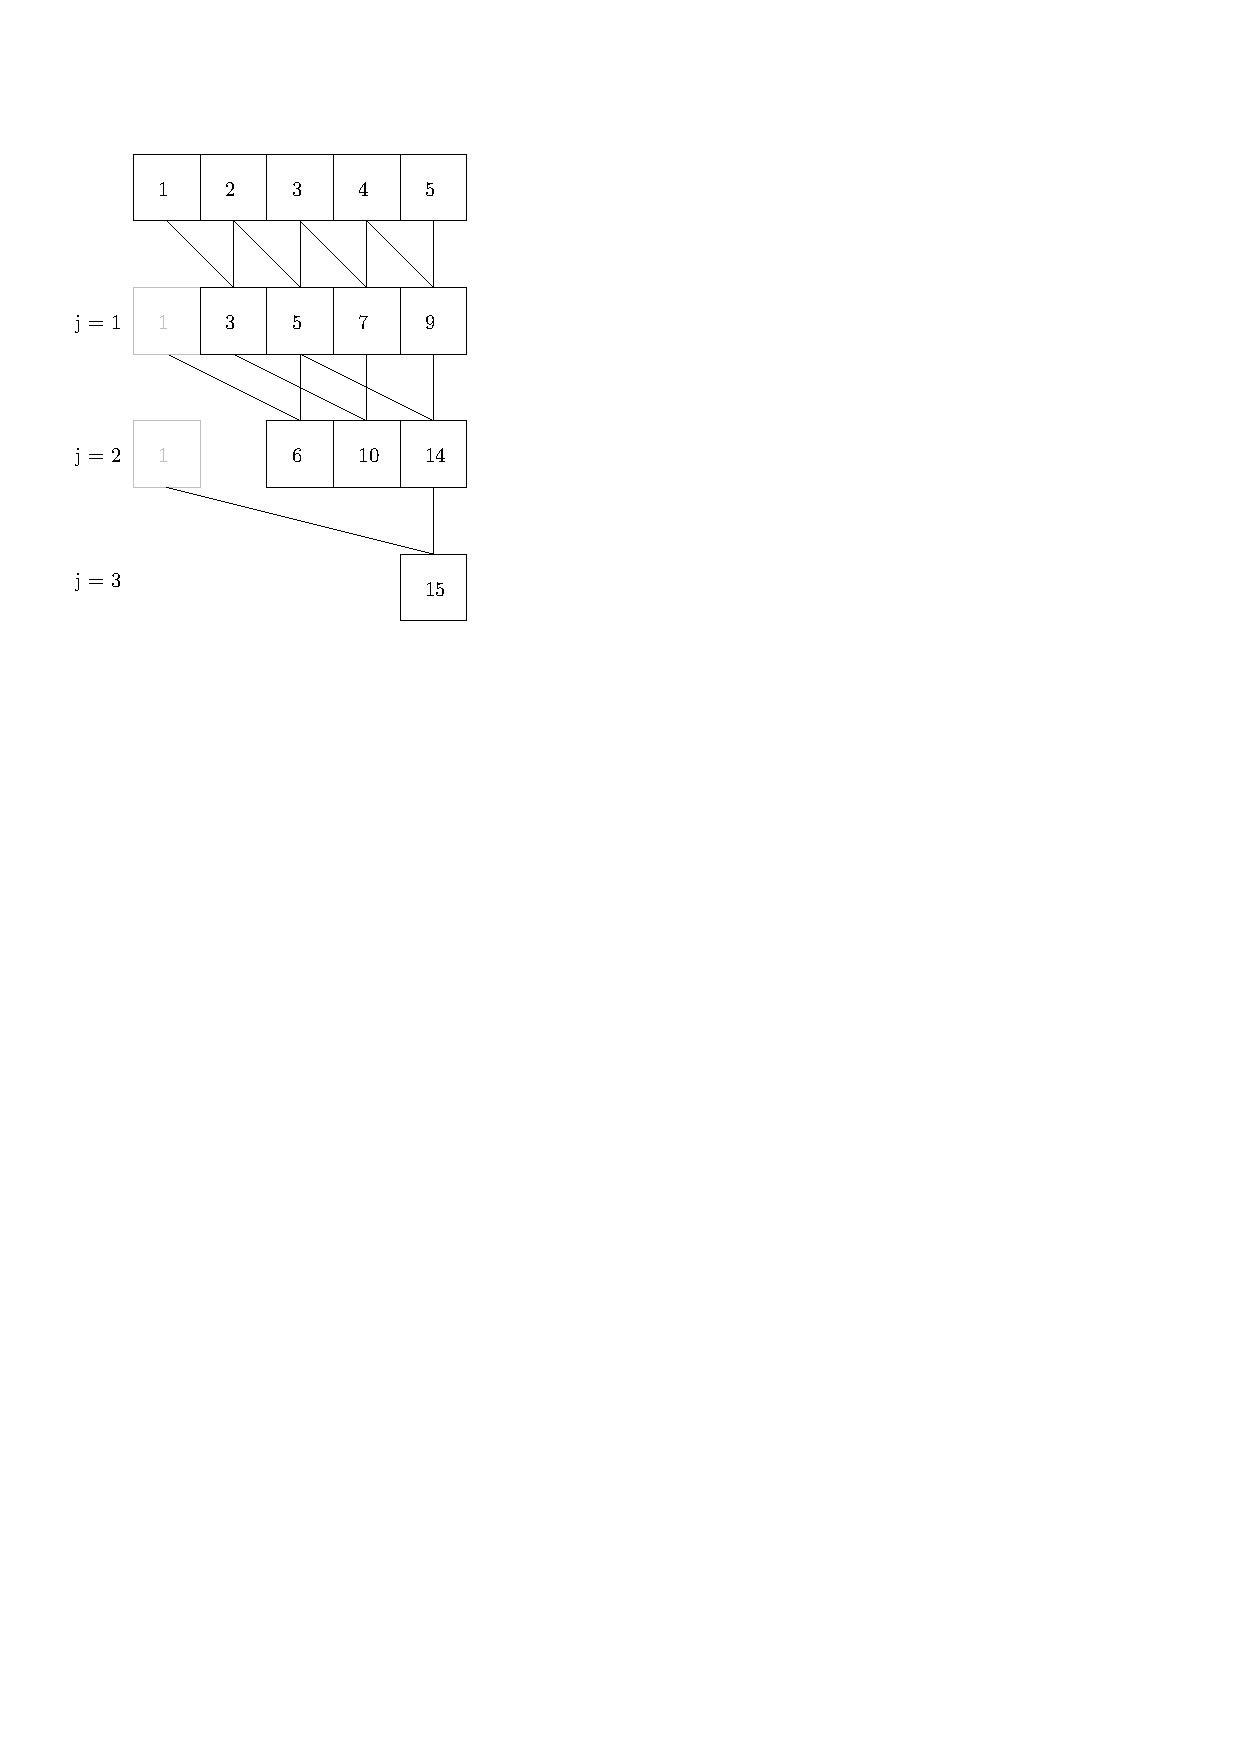
\includegraphics[scale=1]{algo}
\caption{Parallel Scan}
\end{figure}

\begin{tabular}{|p{3cm}|p{6cm}|l|}
\hline
Property&Parallel Scan& Sequential Scan\\
\hline
\hline
\#Opertaions& $\sum\limits_{j=1}^{\log_2n}(n-2^j+1)$& $n-1$\\
\hline

Execution time depending on n/p & $p \ge n -1 : \log_2n$ \newline ca.  $p < n -1 : \log_2n * n/p$& $n-1$\\
\hline

\end{tabular}

While the parallel scan is much faster than the sequential scan, it has  a couple of drawbacks. For instance in distributed memory architectures every node needs to hold it's own copy of the array to be scanned. Additionally after each iteration of j these arrays have to be synchronized. In shared memory architectures that is not the case.

The numerical analysis of the algorithm shown in the table is ignoring communication overhead, as it is assumed that all parallel operations can be executed simultaneously.


\newpage
\textbf{(c) Handling many elements}

The array can be sliced into p (number of processors) parts. On each part one processor does the sequential scan. Afterwards on the last elements of each part a parallel scan with all processors is executed calling the provided scan function. Finally the parts are corrected by using the results of the parallel scan, where each processor adds the associated number to its first scan.

\begin{figure}[hbtp]
\centering
\label{fig:le}
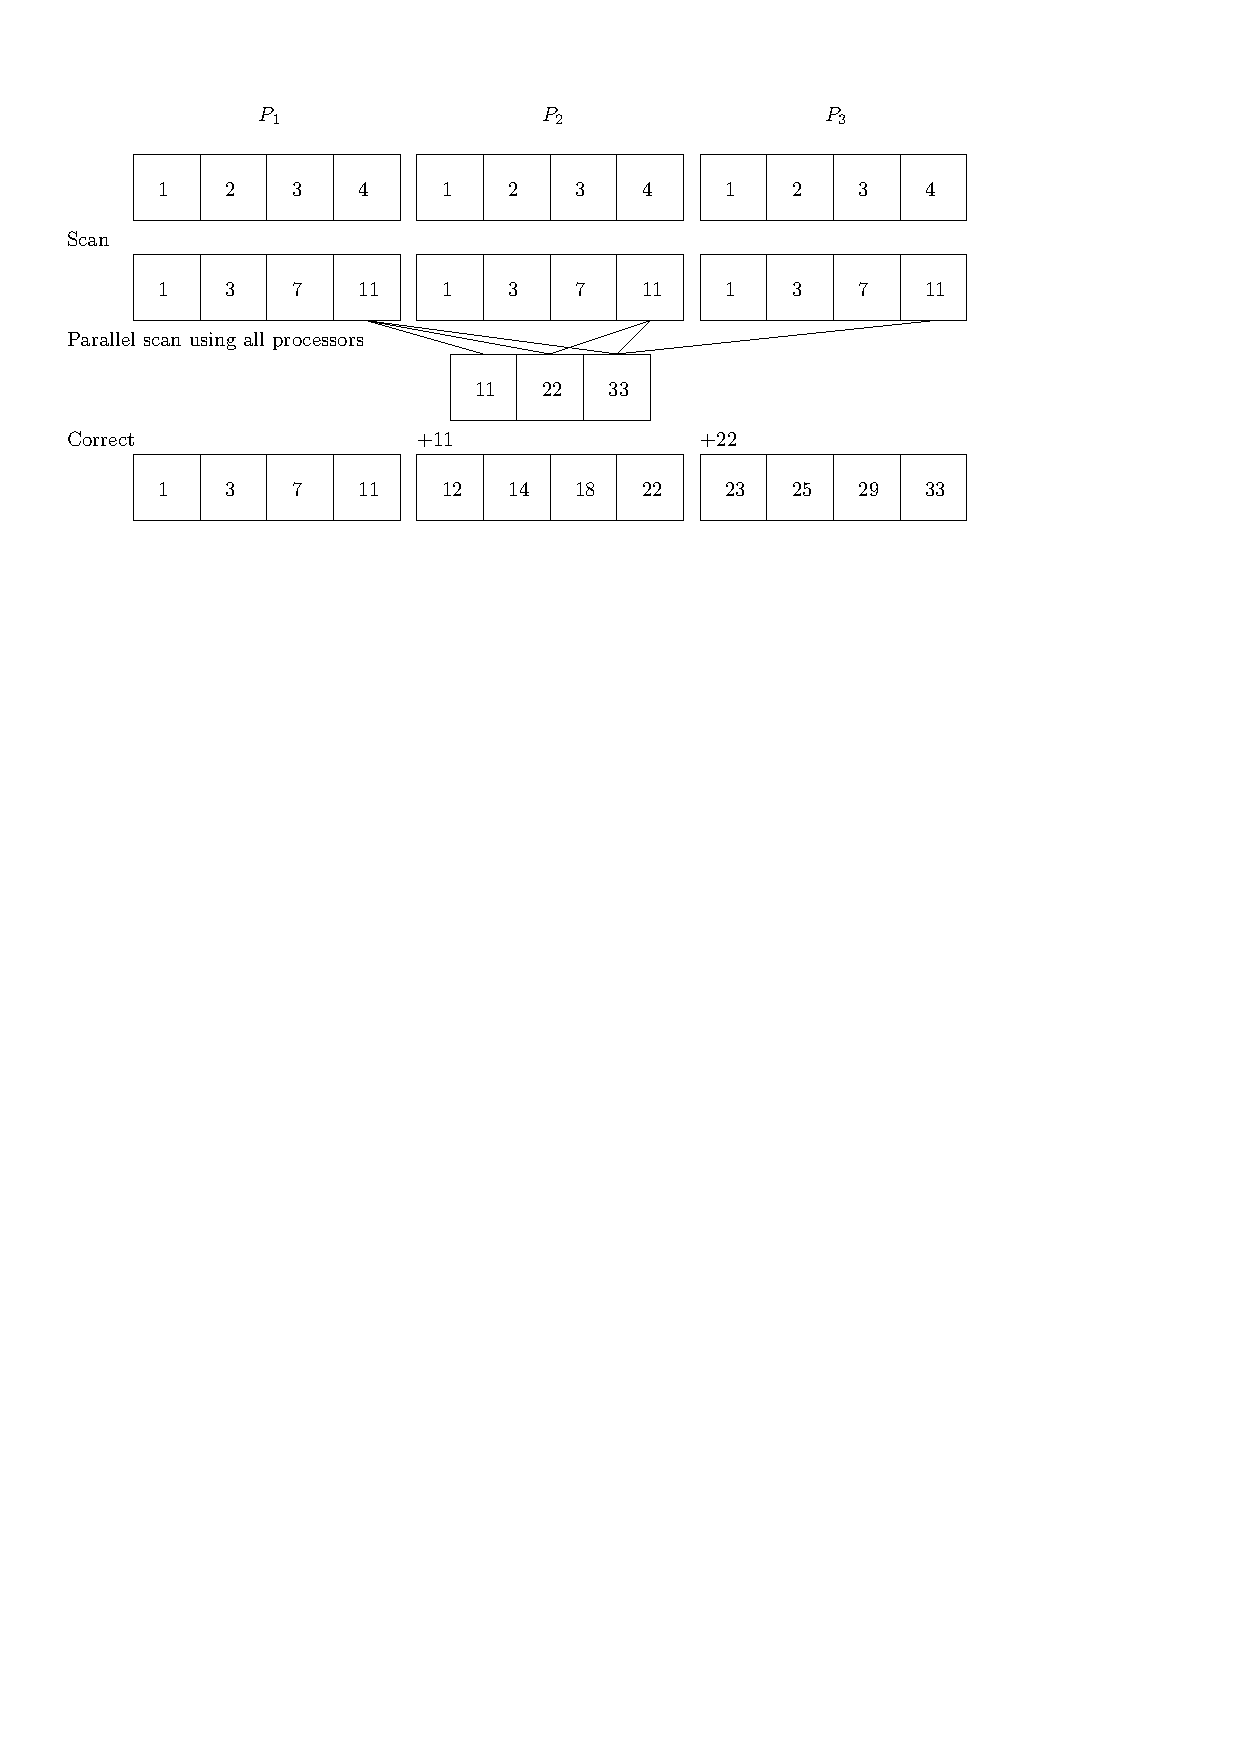
\includegraphics[scale=1]{le}
\caption{Handling many elements having 3 processors}
\end{figure}

Compared to the first algorithm the utilization is better. Having at least as many processors as elements in b, more processors idle with growing j. In c only one processor is idling at the last step.

\newpage
\textbf{(d) Recursion}

The line of thought leads to the algorithm shown in the pseudo code and is visualized in figure 3. The algorithm splits the given array as long as the parts are larger than 2 elements. At that point the primitive task of scanning just 2 elements can be executed. Following this the right half of each split step has to be corrected (named as array.secondPart in the pseudo code). The correction is done by adding the last element of the left half (array.firstPart in pseudo code) to each element of the right half.

The properties of the algorithm make it possible to execute the recursive scan on the two parts after the split individually. So a variable number of tasks can be created. Nevertheless it is necassary to join the execution units before the correction is preformed because the right half (array.secondPart) depends on the result of the left half (array.firstPart). 

The problem of the algorithm is the high overhead caused by the correction step. On the one hand it is an execution barrier that makes it necessary to synchronize the two subtasks at this point. On the other hand especially on distributed memory systems high amount of communication is needed to do the correction. In shared memory systems it is possible to do these operations directly on the array, so the additional communication is not needed.

Pseudo code:
\begin{verbatim}
scan(ref array)
  if(array.size > 2)
    scan(array.firstPart)
    scan(array.secondPart)
    correct(array.secondPart, lastElementOf(array.firstPart))
  else if(array.size == 2)
    array[1] = array[0] + array[1]
	
correct(ref array, correction)
  for(ref element : array)
    element += correction
\end{verbatim}

\begin{figure}[hbtp]
\centering
\label{fig:para_algo}
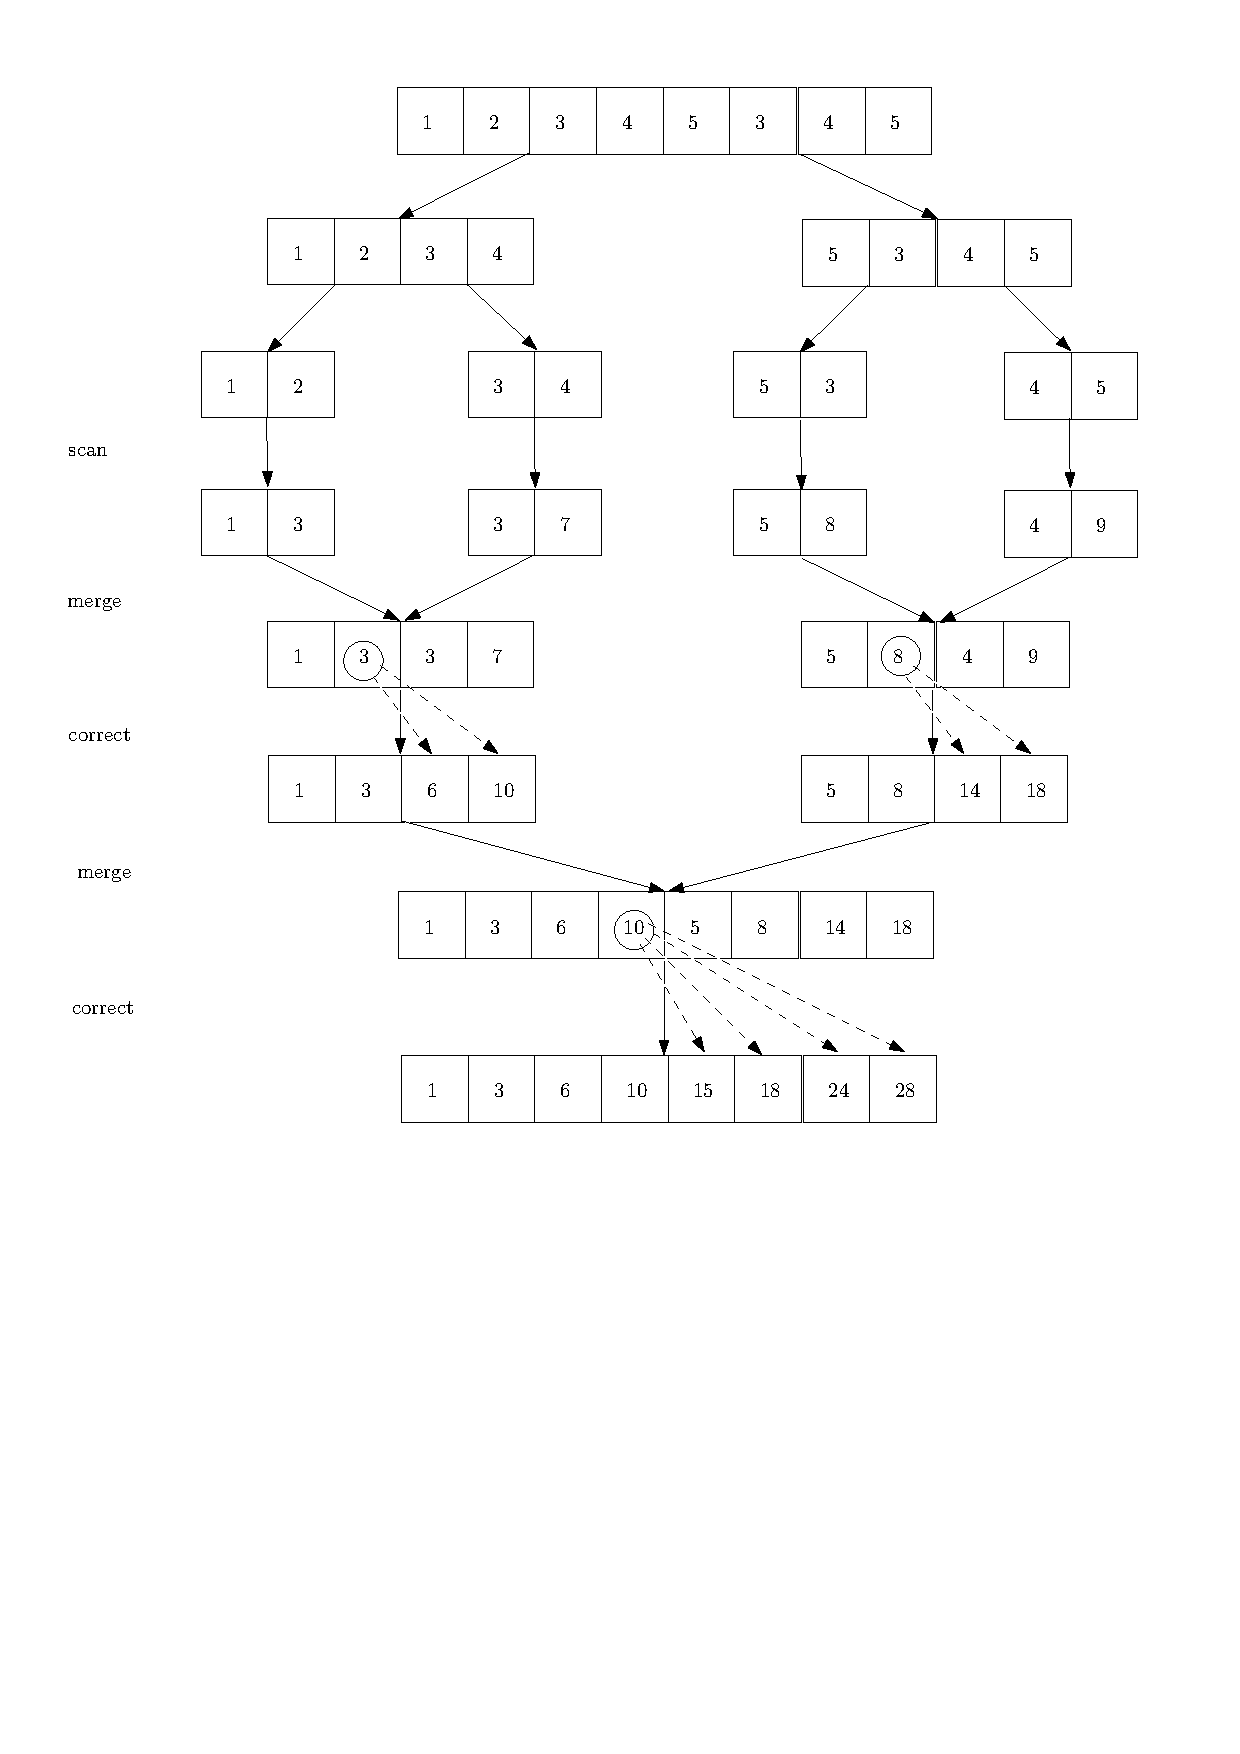
\includegraphics[scale=.75]{recur3}
\caption{Sequence of the recursive scan}
\end{figure}

\section{Exercise 2 - Implementation}

See source in files template.cpp and scan.cl.

\end{document}
